\documentclass[10pt]{scrartcl}

\usepackage[utf8]{inputenc}
\usepackage{tabularx}
\usepackage[ngerman]{babel}
\usepackage[automark]{scrpage2}
\usepackage{amsmath,amssymb,amstext}
%\usepackage{mathtools}
\usepackage[]{color}
\usepackage[]{enumerate}
\usepackage{graphicx}
\usepackage{lastpage}
\usepackage[perpage,para,symbol*]{footmisc}
\usepackage{listings} 
\usepackage[pdfborder={0 0 0},colorlinks=false]{hyperref}
\usepackage[numbers,square]{natbib}
\usepackage{color}
\usepackage{colortbl}

\lstset{numbers=left, numberstyle=\tiny, numbersep=5pt, breaklines=true, showstringspaces=false} 

%changehere
\def\titletext{Praktikum 1 : Modellierung von Raumgestalten}
\def\titletextshort{Praktikum 1}
\author{André Harms, Oliver Steenbuck, Armin Steudte  \\ Carsten Noetzel, Dennis Blauhut, Torben Becker}

\title{\titletext}

%changehere Datum der Übung
\date{26.10.2011}

\pagestyle{scrheadings}
%changehere
\ihead{MI, Thiel-Clemen}
\ifoot{Generiert am:\\ \today}

\cfoot{Oliver Steenbuck \\ André Harms \\  Armin Steudte \\ Carsten Noetzel \\ Dennis Blauhut \\ Torben Becker}


\ohead[]{\titletextshort}
\ofoot[]{{\thepage} / \pageref{LastPage}}

\setlength{\parindent}{0.0in}
\setlength{\parskip}{0.1in}

\begin{document}
\maketitle

\setcounter{tocdepth}{3}
\tableofcontents
\listoffigures
%\lstlistoflistings

\section{Einleitung}

\section{Räumliche Darstellung}
zur Modellierung der der räumlichen Gegebenheiten des Campus Berliner Tor haben wir ein zweidimensionales Raster gewählt.
Hierdurch wird der Campus aus Kacheln zusammen gesetzt, bei dem jede Kachel einem bestimmten Geländemerkmal entspricht.
Dieses ermöglicht es die wesentlichen räumlichen Gegebenheiten auf einer höheren Abstraktionsebene darzustellen, so dass der Detailgrad verringert werden kann.\\
Zur Veranschaulichung des Modellierungskonzepts wurde die Abbildung \ref{img:tile_map} mit Hilfe des Tools \textit{Tiled Map Editor} erstellt. Hier bei wurde beispielhaft ein Ausschnitt des Luftbildes des Campuses modelliert.
Dieses ist in Abbildung \ref{img:google_maps} gekennzeichnet.\\
Um die verschiedenen Geländemerkmale zu visualisieren, haben wir jeden Typ eine Farbe zugeordnet und die jeweiligen Kacheln des Typs in dieser Farbe eingefärbt. Die folgende Tabelle gibt eine Übersicht über die verwendeten Farben und die korrespondierenden Geländemerkmale:

\definecolor{gebaude_durchgang}{rgb}{0.341176471,0.780392157,0.945098039}
\definecolor{gebaude}{rgb}{1,0.921568627,0.474509804}
\definecolor{gruenanlage}{rgb}{0.254901961,0.717647059,0.145098039}
\definecolor{hof}{rgb}{0.050980392,0.48627451,0.690196078}
\definecolor{gehweg}{rgb}{0.68627451,0.709803922,0.682352941}
\definecolor{strasse}{rgb}{0.560784314,0.91372549,0.439215686}
\definecolor{gehweg_sek}{rgb}{0.623529412,0.490196078,0.203921569}

\begin{tabular}{|c|c|}
\hline 
\textbf{Farbe} & \textbf{Geländemerkmal} \\ 
\hline 
\cellcolor{gebaude} & Gebäude \\
\hline 
\cellcolor{gebaude_durchgang} & Gebäudedurchgang\\
\hline 
\cellcolor{gruenanlage} &  Grünanlage\\ 
\hline 
\cellcolor{hof} &  Hof\\ 
\hline 
\cellcolor{gehweg} & Gehweg\\ 
\hline 
\cellcolor{gehweg_sek} & Sekundär Gehweg\\
\hline 
\cellcolor{strasse} & Straße\\ 
\hline 
\end{tabular} 


      \begin{figure}[htbp]
        \centering
                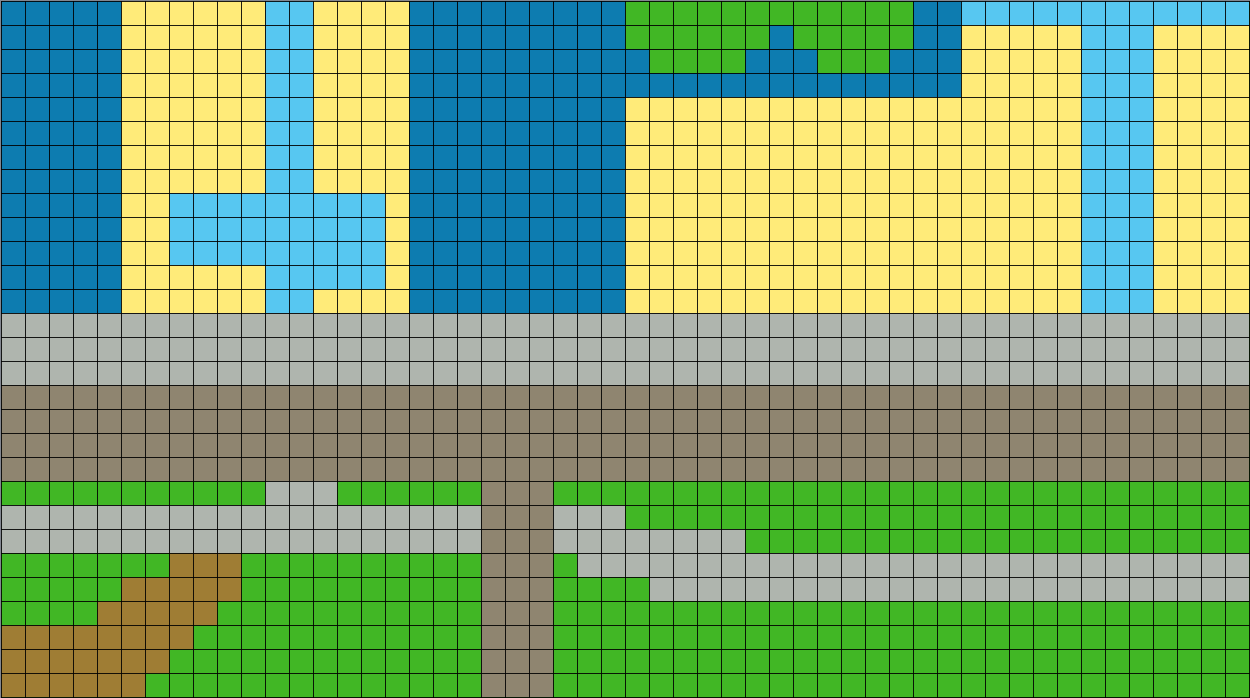
\includegraphics[scale=0.5]{img/tile_map_campus_pic}
        \caption{Ausschnitt von Campus als \glqq Tilebased Map\grqq{}}
        \label{img:tile_map}
        \end{figure}  
        
        
      \begin{figure}[htbp]
        \centering
                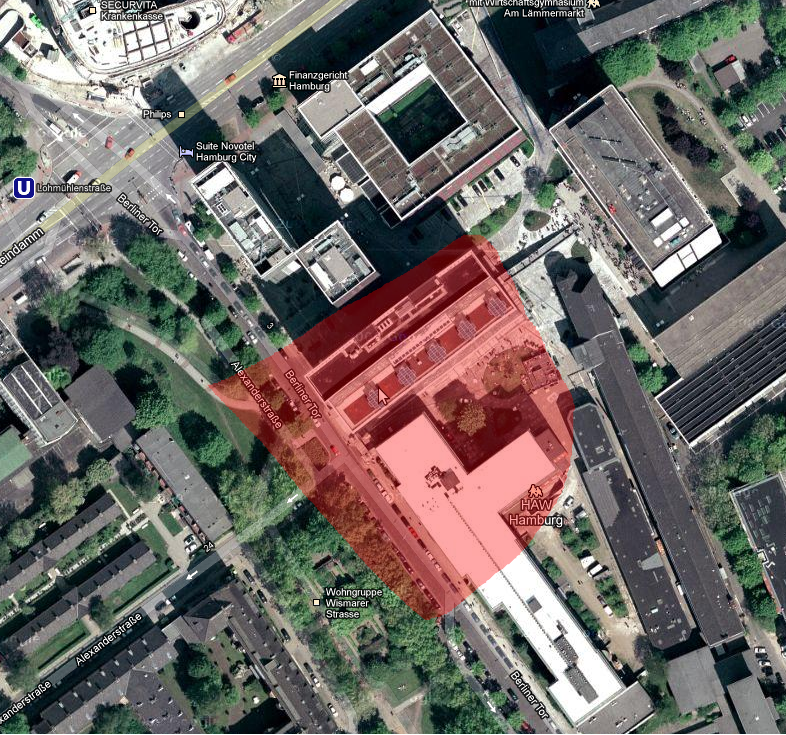
\includegraphics[scale=0.5]{img/google_maps}
        \caption{Ausschnitt Google-Maps}
        \label{img:google_maps}
        \end{figure}  
        
        
        Um andere Aspekte als die räumlichen Gegebenheiten modellieren zu können, ist es möglich ein Layerkonzept zu verwenden. Hierbei werden die gewünschten Eigenschaften auf anderen Schichten modelliert. Diese Schichten lassen sich dann entsprechend verwenden und auswerten.
Sollte sich herausstellen, dass eine 3-dimensionale Modellierung besser geeignet ist, besteht die Möglichkeit, zu einem 3-D Modell zu wechseln. Hier werden zusätzliche Eigenschaften nicht mehr in Layer modelliert sondern in parallelen Räumen, sogenannte Spaces.

\section{Entitäten}

	\subsection{Beschreibungen}
	Nachfolgend folgen die Beschreibungen der einzelen Entitäten. Diese sind zur besseren Übersicht in drei Gruppen untergliedert. Die Gruppe \verb!Verkehr! enthält alle diejenigen Entitäten, die zur Verwaltung des Verkehrsflusses auf dem Campus genutzt werden können. Dabei ist mit Verkehr, sowohl der Fußgängerverkehr, als auch der Kraftverkehr gemeint.
	Die Gruppe \ver!Inventar! hingegen, enthält alle diejenigen Entitäten die halbwegs bewegbar auf dem Campusgelände vertelt werden können. Die letzte Gruppe der \verb!Architektur! beinhaltet Entitäten die feste Strukturen darstellen und nicht beweglich sind.\\
	Allen Entitäten leiten von der Klasse \verb!Object! ab und haben damit eine Positon auf dem Campusgelände und eine Dimension, die ihre Größe angibt. Jedem Objekt sind Einflussfaktoren zugeornet, die auf der Metaebene der Modells analysiert werden sollen. Dies sind \verb!Vergnügen!,
	\verb!Sozialisierung!, \verb!Sicherheit! und \verb!Produktivität! die unter Abschnitt \ref{sec:Ebenen} vorgestellt werden.
	
	\subsubsection{Verkehr}
	\begin{tabular}{|c|c|}
\hline Entität & Beschreibung \\ 
\hline
\hline Grünfläche &  \\ 
\hline Wege &  \\ 
\hline Parkplätze &  \\ 
\hline Fahrradstellplätze &  \\ 
\hline Verkehrszeichen &  \\ 
\hline Ampel &  \\ 
\hline 
\end{tabular} 

	\subsubsection{Inventar}
\begin{tabular}{|c|c|}
\hline Entität & Beschreibung \\
\hline
\hline Beleuchtungsquelle &  \\ 
\hline Bank &  \\ 
\hline Aschenbecher &  \\ 
\hline Mülleimer &  \\ 
\hline Abwasserschacht &  \\ 
\hline WLAN AP &  \\ 
\hline 
\end{tabular}

	\subsubsection{Architektur}
\begin{tabular}{|c|c|}
\hline Entität & Beschreibung \\
\hline	
\hline Gebäude &  \\ 
\hline Mauer &  \\ 
\hline Eingang &  \\ 
\hline 
\end{tabular} 

	\subsection{Klassendiagramm}
	Im folgenden wird das sich aus der vorhergehenden Sektion ergebende Klassendiagramm visualisiert (hier mit VisualParadigm).
	Hier wurde, zum Zweck der Übersichtlichkeit darauf verzichtet darzustellen, dass alle Entitäten von \verb!Objekt! ableiten.
      \begin{figure}[Htp]
        \centering
                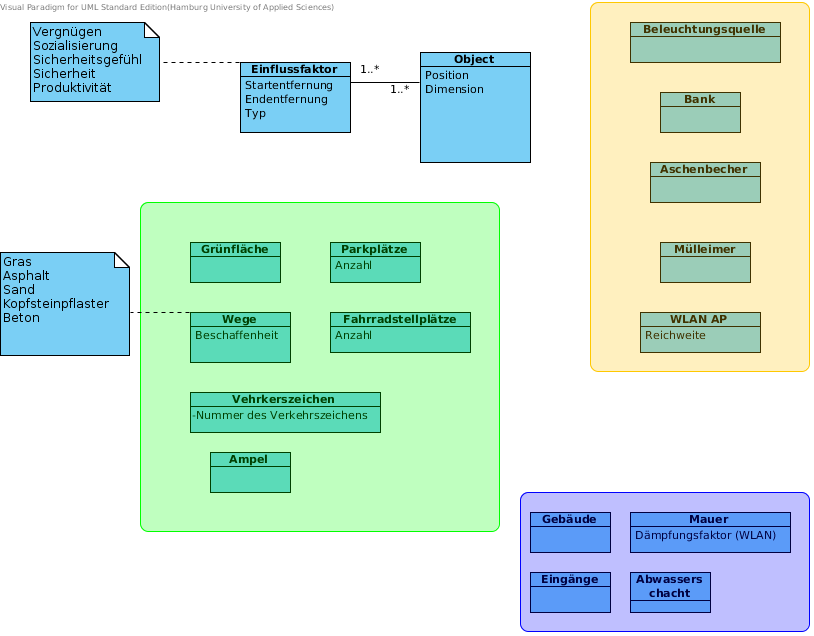
\includegraphics[scale=0.6]{img/ClassDiagram.png}
        \caption{Klassendiagramm}
        \label{img:classDiagram}
        \end{figure}  	
	 
	 

\section{Ebenen}\label{sec:Ebenen}
Eine Ebene ist eine Abstrahierung von Messungen, gef\"uhlten Werten bzw. Erfahrungswerten. Diese Werte werden auf einer Karte in Zonen dargestellt. Eine Zone besteht dabei aus mehreren quadratischen Feldern in der r\"aumlichen Darstellung. Dabei ist der Wert in der Mitte der Zone am h\"ochsten und flacht zum Rand der Zone hin ab. Eine Alternative w\"are, dass ein Wert pro Feld dargestellt wird.
\newline Der Wert eines Feldes wird im prozentualen Anteil des maximal m\"oglichen Wertes angegeben und dem entsprechend mit einer Farbe verbunden, die anzeigt, ob etwas gut oder schlecht ist. Als Beispiel die Sicherheit, die auf einer Wiese deutlich h\"oher sein d\"urfte, als auf einer sechs spurigen Stra\"se in einer Gro\"sstadt.

\subsection{Sicherheit}
Die Sicherheitsebene vergibt Werte f\"ur einzelne Bereiche in der r\"aumlichen Darstellung. Eine farbliche Darstellung der einzelnen Bereiche steht f\"ur den dahinter liegenden Wert. Je r\"oter der Bereich ist, desto gef\"ahrlicher ist es. Und je gr\"uner es wird, um so sicherer f\"uhlen sich Menschen. Dabei steigt zum Beispiel das Gef\"uhl der Sicherheit, je weiter man sich von der Stra\"se fortbewegt oder auf der Stra\"se, wenn mittels eines Zebrastreifens f\"ur eine Erh\"ohung der Sicherheit gesorgt wird.
\newline Die Sicherheit kann direkten Einfluss nehmen auf das Wohlbefinden der Personen. Denn trotz eines guten Wohlbefindens, kann dieses gemindert werden, wenn die Sicherheit sinkt, indem eine kritische Situation entsteht.

\subsection{Feel Good}
In der Feel Good-Ebene wird das Befinden der Personen dargestellt. Auch in dieser Ebene wird die gleiche farbliche Gestaltung verwendet. Ist ein Bereich gr\"un bzw. wird gr\"uner, f\"uhlt sich die Person umso wohler. Ist der Bereich rot resp. wird r\"oter, f\"uhlt sich die Person unwohler. Das Wohlbefinden einer Person kann von unterschiedlichen Faktoren beeinflusst werden, wie z.B. die N\"ahe zur Stra\"se, Anzahl der Fahrzeuge auf der Straße oder von vorhandenen Gr\"unfl\"achen bzw. Aufenthaltsbereichen mit oder ohne Sitzgelegenheiten.

\subsection{Durchfluss}
In dieser Ebene wird der maximal m\"ogliche Durchfluss eines gewissen Bereiches dargestellt. Es wird eine farbliche Darstellung gew\"ahlt, bei der gr\"un bedeutet, dass viele Personen pro Zeit diesen Bereich passieren k\"onnen respektive rot, wenn eher wenig Personen pro Zeit den Bereich durchqueren k\"onnen.
\newline Die Erfahrungen bzw. Erkenntnisse dieser Ebene k\"onnen auch direkten Einfluss auf die Feel Good- und Sicherheitsebene haben. Ist an einer gewissen Stelle der Karte der maximal m\"ogliche Durchfluss gering und es ist bekannt, dass zu gewissen Zeiten aber viele Menschen durch diesen Bereich wollen, k\"onnte dies einen direkten negativen Einfluss auf die Sicherheit und das Wohlbefinden liefern und deren Werte verschlechtern.


\end{document}

